%%%%%%%%%%%%%%%%%%%%%%%%%%%%%%%%%%%%%%%%%%%%%%%%%%%%%%%%%%%%%%%%%%%%%%%%%%%%%%%%%%%%%%%%%%%%%%%%%%%%%%%%%%%%%%%%%%%%%%%%%%%%%%%%%%%%%%%%%%%%%%%%%%%%%%%%%%%%%%%%%%%%%%%%%%%%%%%%%%%%
%%%%%%%%%%%%%%%%%%%%%%%%%%%%%%%%%%%%%%%%%%%%%%%%%%%%%%%%%%%%%%%%%%%%%%%%%%%%%%%%%%%%%%%%%%%%%%%%%%%%%%%%%%%%%%%%%%%%%%%%%%%%%%%%%%%%%%%%%%%%%%%%%%%%%%%%%%%%%%%%%%%%%%%%%%%%%%%%%%%%
%%%%%%%%%%%%%%%%%%%%%%%%%%%%%%%%%%%%%%%%%%%%%%%%%%%%%%%%%%%%%%%%%%%%%%%%%%%%%%%%%%%%%%%%%%%%%%%%%%%%%%%%%%%%%%%%%%%%%%%%%%%%%%%%%%%%%%%%%%%%%%%%%%%%%%%%%%%%%%%%%%%%%%%%%%%%%%%%%%%%
\FloatBarrier
\chapter{General search strategy}
\label{sec:GeneralSearchStrategy}

At the LHC, there are several possible chargino production channels. 
Chargino pairs can be produced through a photon or a $Z$-boson exchange. 
The chargino then decays via a virtual $W$-boson to the lightest neutralino and a fermion pair (\eg a pion). 
This process is illustrated in the Feynman diagram in Fig.~\ref{fig:FeynmanDiagram}.
Other possible chargino pair production channels include the exchange of a supersymmetric Higgs boson or a t-channel squark exchange (Fig.~\ref{fig:FeynmanDiagramProductionCharginoPair}).

Apart from pair production, charginos can be produced via the chargino-neutralino channel. 
On tree-level, there exist two production mechanisms: the s-channel $W$-boson exchange and the t-channel squark exchange (Fig.~\ref{fig:FeynmanDiagramProductionCharginoNeutralino}).
\begin{figure}[!b]
  \centering 
  \begin{tabular}{c}
    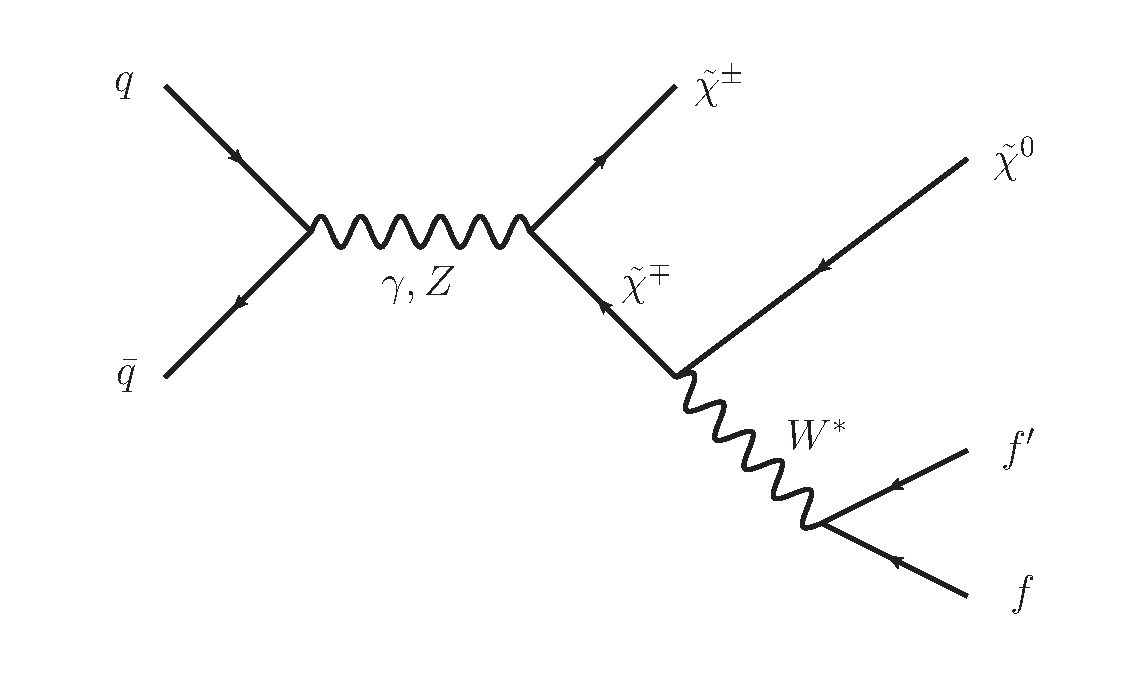
\includegraphics[width=0.75\textwidth]{figures/analysis/ChiChi_ProductionAndDecay.pdf}
  \end{tabular}
  \caption{Feynman diagram of chargino pair production via gamma or $Z$-boson exchange and the subsequent decay via a virtual $W$-boson.}
  \label{fig:FeynmanDiagram}
\end{figure}

\begin{figure}[!h]
  \centering 
  \begin{tabular}{c}
    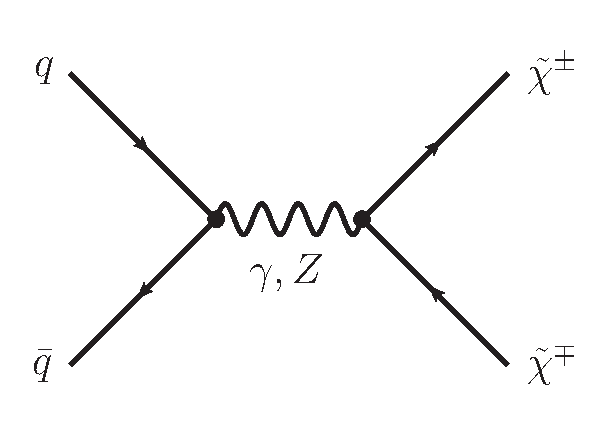
\includegraphics[width=0.33\textwidth]{figures/analysis/ChiChi_GammaZ.pdf}
    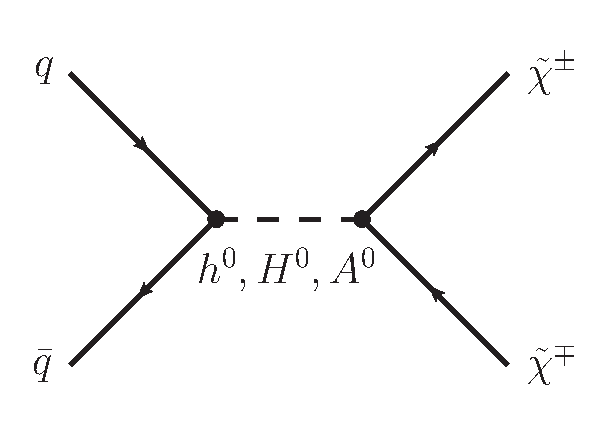
\includegraphics[width=0.33\textwidth]{figures/analysis/ChiChi_Scalar.pdf}
    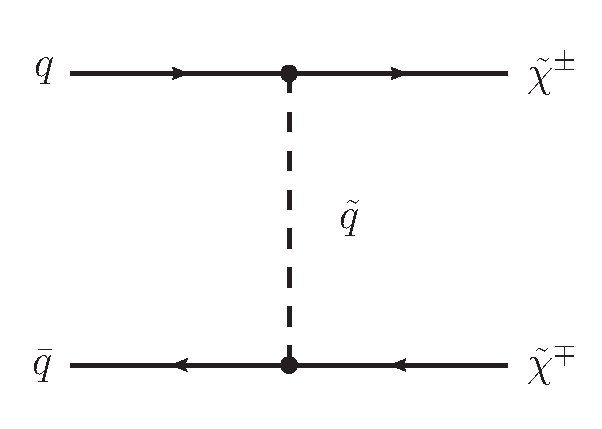
\includegraphics[width=0.33\textwidth]{figures/analysis/ChiChi_Squark.pdf}
  \end{tabular}
  \caption{Main tree-level diagrams for chargino pair production.}
  \label{fig:FeynmanDiagramProductionCharginoPair}
\end{figure}

\begin{figure}[!h]
  \centering 
  \begin{tabular}{c}
    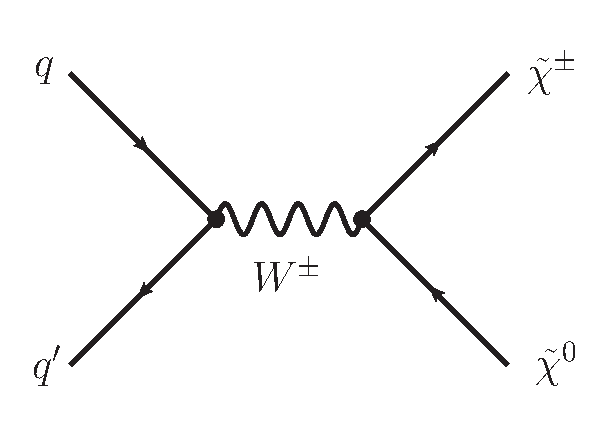
\includegraphics[width=0.33\textwidth]{figures/analysis/ChiChi0_WBoson.pdf}
    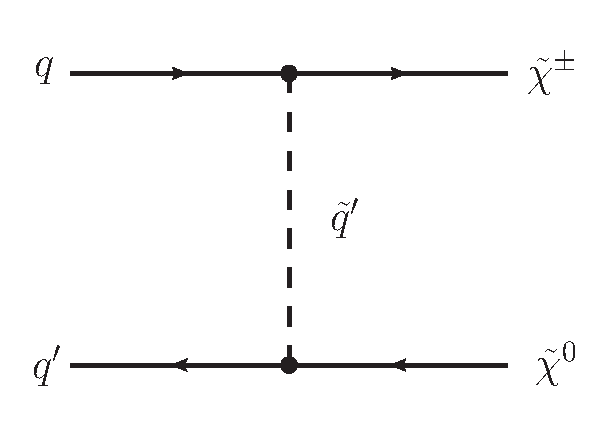
\includegraphics[width=0.33\textwidth]{figures/analysis/ChiChi0_Squark.pdf}
  \end{tabular}
  \caption{Main tree-level diagrams for chargino neutralino production.}
  \label{fig:FeynmanDiagramProductionCharginoNeutralino}
\end{figure}
Alternatively, charginos can be produced via strong production modes, \ie in cascade decays of new heavy particles, such as gluinos or squarks.
In the here presented search, the focus is, however, put on the electroweak production channels: chargino pair and chargino-neutralino production.\\


When searching for supersymmetric models with long-lived \chipm, the strategy is of course highly dependent on the actual lifetime of the chargino. 
For long lifetimes, the chargino can reach the muon chambers and can be reconstructed as a muon even despite a longer time-of-flight~\cite{bib:CMS:HSCP_7TeV}. 
For lower lifetimes, the chargino can already decay inside the detector (\eg the tracker), and hence can not be reconstructed as a muon but leads to an isolated, potentially disappearing track in the tracker. 
The detector signatures of these two scenarios are visualised in Fig.~\ref{fig:CharginoPaiEventDisplay}, where simulated chargino-chargino events are shown in a cross-sectional view of the CMS detector.
\begin{figure}[!t]
  \centering 
  \begin{tabular}{c}
  \begin{subfigure}{0.31\textwidth}
    \frame{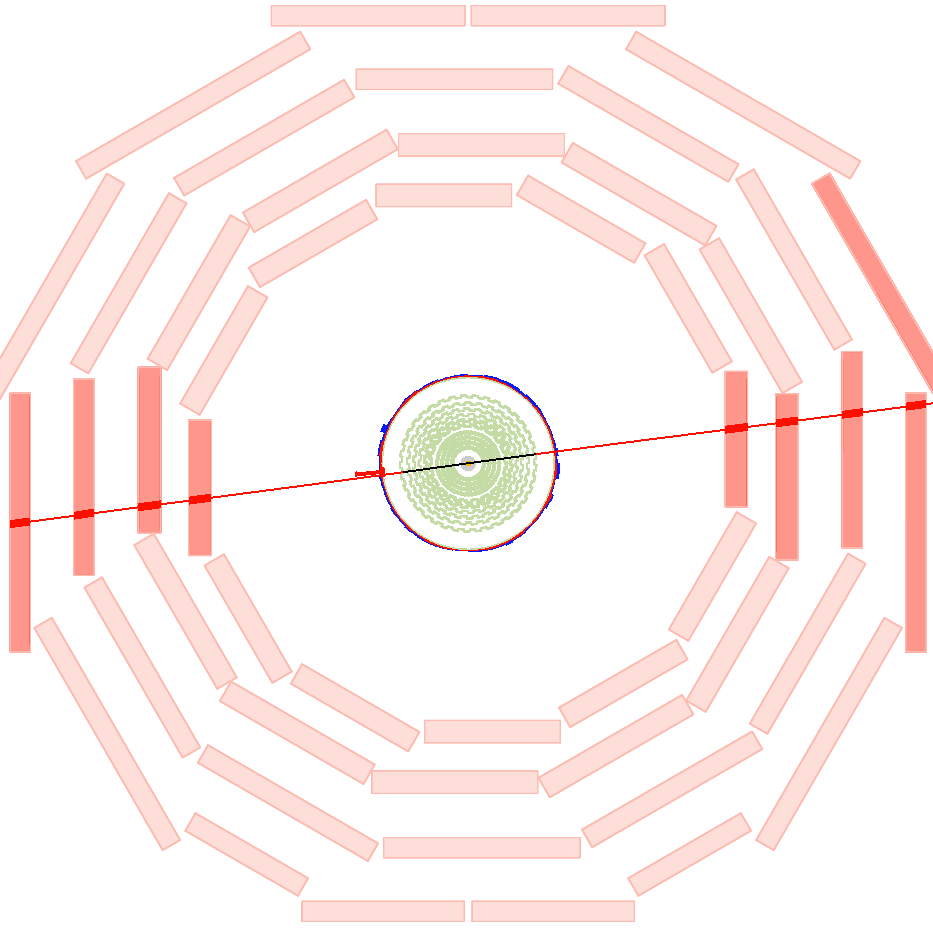
\includegraphics[width=0.99\textwidth]{figures/analysis/MotivationAndGeneralSearchStrategy/CharginoPairEvent_ctau_10000cm_lumi_1_event_12015.png}}
      \caption{}
  \end{subfigure} 
  \begin{subfigure}{0.31\textwidth}
    \frame{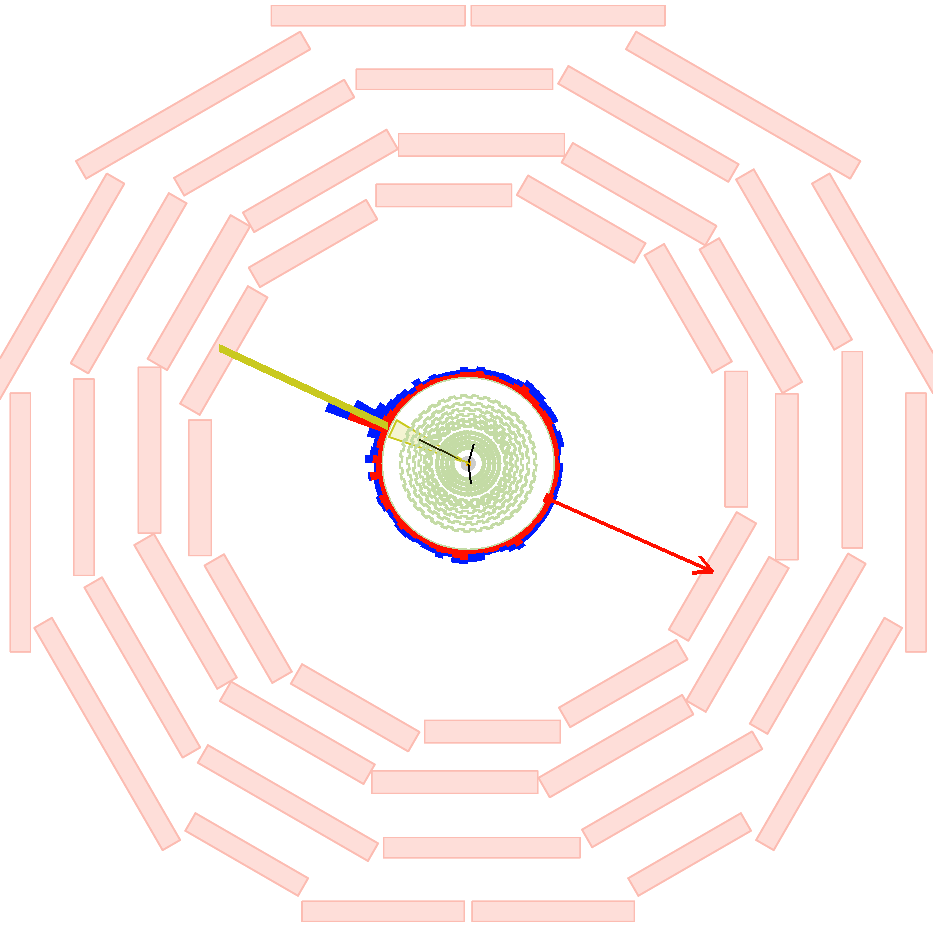
\includegraphics[width=0.99\textwidth]{figures/analysis/MotivationAndGeneralSearchStrategy/CharginoPairEvent_ctau_50cm_lumi_1_event_11024.png}}
      \caption{}
  \end{subfigure} 
  \begin{subfigure}{0.31\textwidth}
      \frame{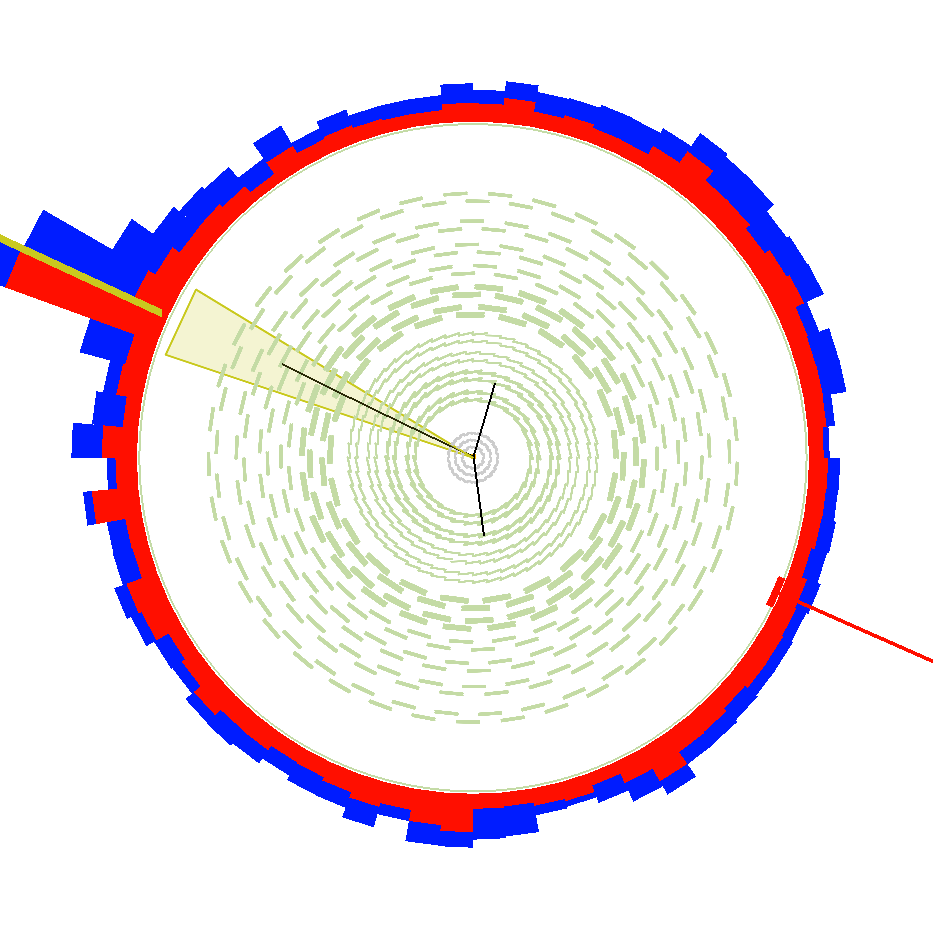
\includegraphics[width=0.99\textwidth]{figures/analysis/MotivationAndGeneralSearchStrategy/CharginoPairEvent_ctau_50cm_lumi_1_event_11024_Zoom.png}}
      \caption{}
  \end{subfigure} 
  \end{tabular}
  \caption{Visualisation of possible signatures of a chargino pair produced with a lifetime of $\ctau = 10\,\text{m}$ (a) and a lifetime of $\ctau = 0.5\,\text{m}$ (b and c). 
           The muon chambers are the outer layers of the detector and are depicted as red boxes.
           The black lines represent the reconstructed chargino tracks.
           The right picture (c) is a zoom of the middle picture (b). 
           Here, only the cross-section of the tracker (green wavy lines for the strip and grey lines for the pixel) is displayed. The red arrow shows the missing transverse energy in the event.
           The red (blue) towers correspond to the energy deposition in the ECAL (HCAL).
           The ISR jet in the middle and right picture is indicated as a yellow line.} 
  \label{fig:CharginoPaiEventDisplay}
\end{figure}
In the left picture of Fig.~\ref{fig:CharginoPaiEventDisplay}, both charginos are reconstructed as muons, which can be seen by the energy deposition in the muon chambers.
In the middle and right pictures both charginos have a lower lifetime of $\ctau=0.5\,$m and thus are only visible as tracks in the tracker, where both trajectories end inside the silicon strip tracker (by coincidence the tracks are equally long).
Since this analysis targets a search for Supersymmetry with charginos of lifetimes between $\ctau \approx 1\,\text{cm} - 10\,\text{cm}$, the charginos decay rather early in the detector, possibly even in the inner layers of the tracker.
%Thus, the signature of chargino events consists of isolated, short tracks that have large ionisation losses due to high chargino masses and the signatures of the decay products, \ie of a neutralino and a fermion pair. 
Thus, the signature of chargino events consists of isolated, short tracks and the signatures of the decay products, \ie of a neutralino and a fermion pair. 

In case of R-parity conservation, one of the chargino decay products, the neutralino, is stable and weakly interacting, thus traversing the detector without leaving any further signature.
%The missing transverse energy of the neutralino is balanced by the missing transverse energy of the second produced SUSY particle.
%This is either a neutralino or the decay products of the chargino in events with chargino pairs. 

The signature of the other decay product, the fermion pair, can in principle be used to select chargino events. 
However, for mass-degenerate charginos, it can be very hard or even impossible to detect these fermions as will be explained in detail in the next paragraph.

First of all, the fermionic decay product (\eg a pion) can usually not be reconstructed because it does not originate from the primary vertex.
Secondly, it is very low in momentum because of the mass-degeneracy between \chipm and \chiO.
The typical momentum of a pion originating from a chargino to neutralino decay in the \chipm rest frame is of the order 
\begin{equation}
p_{\pi}\sim \sqrt{ \left( m_{\chipm} - m_{\chiO} \right)^2 - m_{\pi}^2}.
\end{equation}
%As the \chipm is rather slow for higher masses this is a good approximation also in the detector rest frame.
For a mass gap between \chipm and \chiO of 150\mev, the \pt distribution of the resulting pion peaks \mbox{at $\sim$ 100\,\mev} and ends at \mbox{\pt $\sim 400\,$\mev} in the laboratory frame (Fig.~\ref{fig:ptOfPions}).
\begin{figure}[!t]
  \centering 
 \vspace{10pt}
  \begin{tabular}{c}
    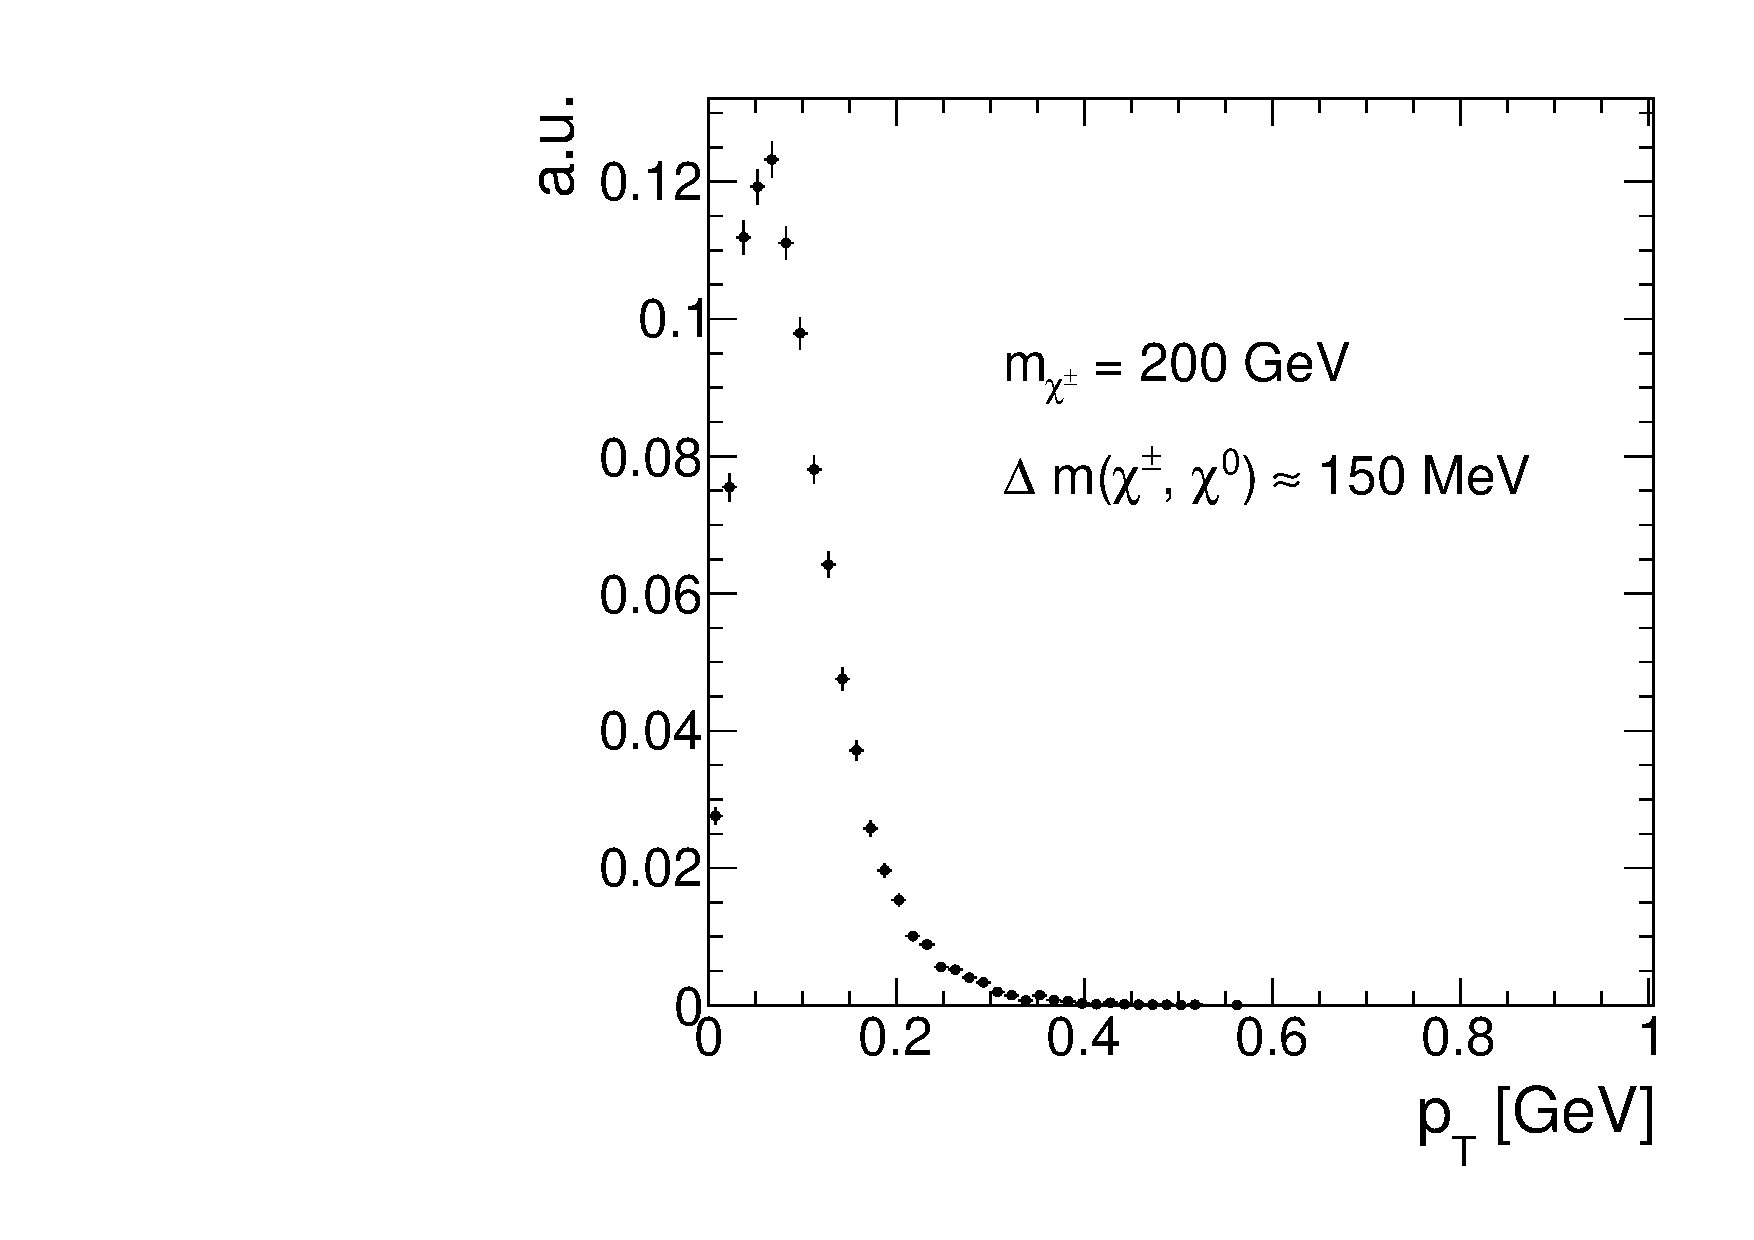
\includegraphics[width=0.49\textwidth]{figures/analysis/PtOfPions.pdf}
  \end{tabular}
  \caption{Transverse momentum distribution of pions coming from charginos decay into a neutralino with a mass gap of 150\mev.}
  \label{fig:ptOfPions}
\vspace{80pt}
\end{figure} 

If the transverse momentum of a particle is very low, the particle trajectory is much more bended compared to a particle with higher \pt (see Fig.~\ref{fig:KinkedTrack} for illustration).
Due to this bending, the track reconstruction efficiency of particles with a transverse momentum below 1\gev decreases rapidly, reaching around 40\% for isolated pions with a \pt of 100\mev~\cite{bib:CMS:tracking_8TeV}. 
Furthermore, for pions that are not produced in the primary vertex, this reconstruction efficiency will be even smaller.
It is therefore impossible to rely on a reconstruction of the fermionic chargino decay products in this analysis.
\begin{figure}[!b]
  \centering 
  \begin{tabular}{c}
    \frame{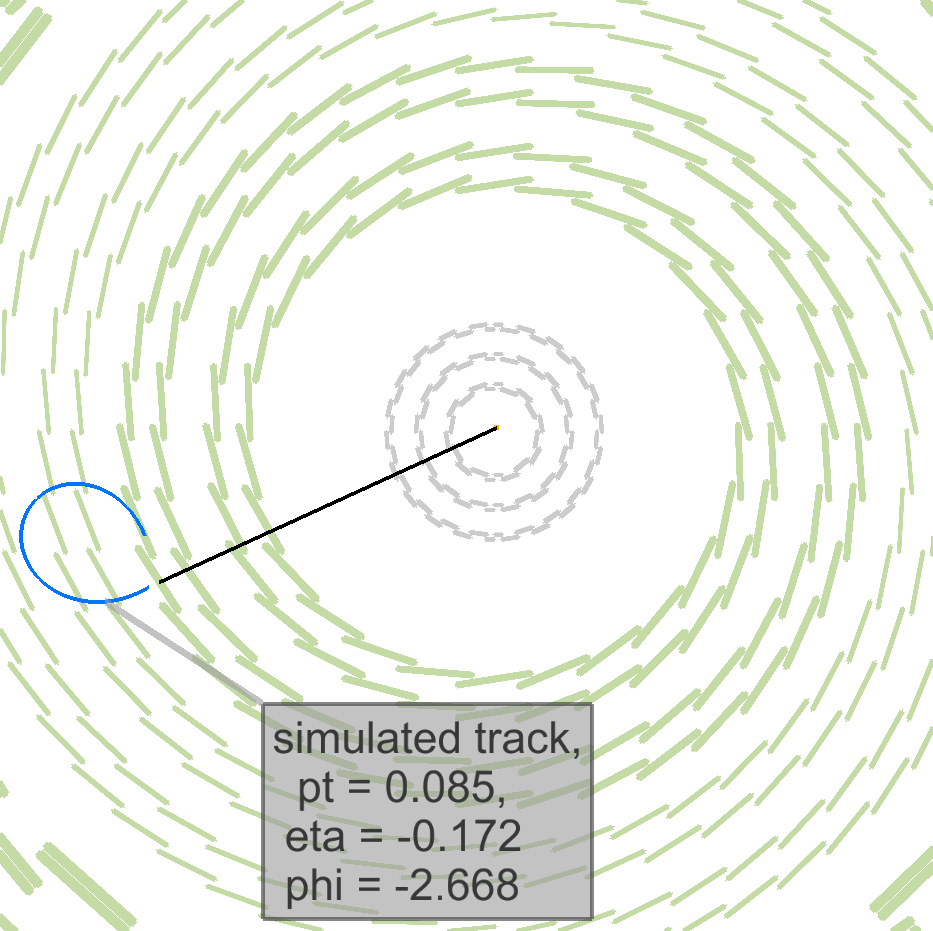
\includegraphics[width=0.4\textwidth]{figures/analysis/MotivationAndGeneralSearchStrategy/BendedPionTrack.png}}
    %\frame{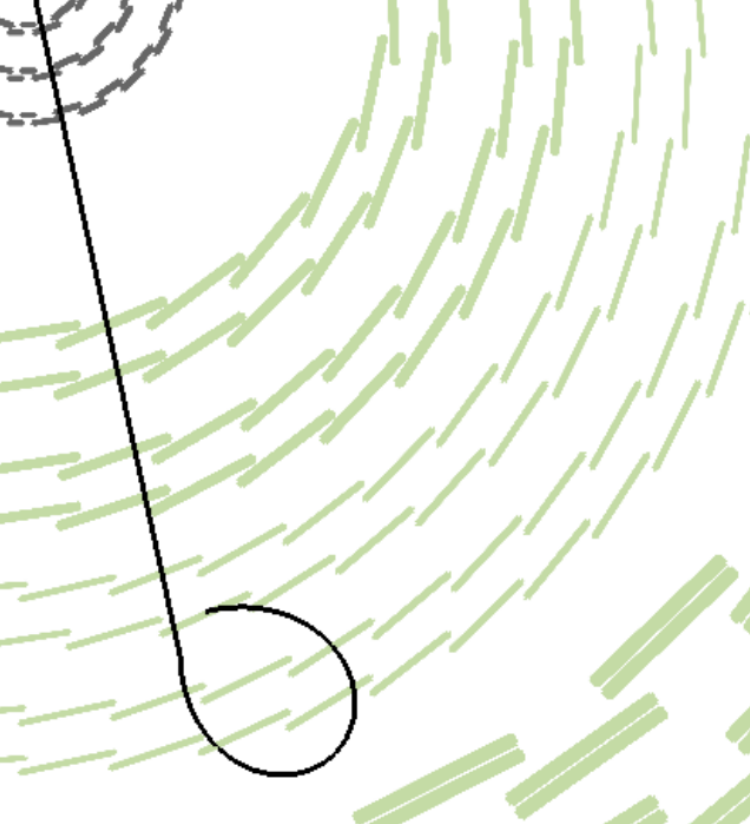
\includegraphics[width=0.30\textwidth]{figures/analysis/KinkedTrackZoom_Quadrat.png}}
  \end{tabular}
  \caption{Cross-sectional view of the silicon strip tracker (green lines) and silicon pixel tracker (grey lines). A simulated chargino track (black line) decays to a pion (bended blue line) with a \pt of $\sim 85\mev$ and a neutralino (not visible).}
  \label{fig:KinkedTrack}
\end{figure} 

In summary, since an early decaying chargino is not reconstructed as a PF particle, the event signature of a chargino-pair or a chargino-neutralino event consists only of one (or two) - potentially - disappearing track. 
Such a signature is very difficult to detect, especially since CMS doesn't offer a dedicated track trigger so that triggering on the chargino track is impossible.


In order to search for such signatures, one therefore needs to trigger on other, less obvious properties of chargino events. 
This analysis takes advantage of higher order contributions to the Feynman diagrams shown in Figs.~\ref{fig:FeynmanDiagramProductionCharginoPair} and~\ref{fig:FeynmanDiagramProductionCharginoNeutralino}, resulting in initial state radiation (ISR).
If the initial quarks radiate a high \pt gluon, the resulting jet can be detected and can offer a possibility to search for events with - apart from the ISR jet - nothing more than isolated tracks.
Furthermore, the non-detection of the chargino's decay products plus a high \pt ISR jet leads to missing transverse energy (MET) in the event. 
Exploiting these two circumstances, it is possible to detect chargino-pair or chargino-neutralino events with the help of Jet+MET triggers.

Since Jet+MET triggers are not very specific for chargino events, it is important to identify further track properties that can be used to select chargino candidates.
One distinctive property of charginos compared to SM particles is their high mass. 
Therefore, charginos can be identified by selecting high \pt tracks. 
Furthermore, the energy loss per path length (\dedx) depends quadratically on the particle mass for low velocities ($0.2<\beta\gamma<0.9$):
\begin{equation}
\langle\frac{dE}{dx}\rangle = K \frac{m^2}{p^2} +C
\end{equation}
Therefore, \dedx constitutes a very nice discriminating variable for massive particles like charginos against SM particles.
The selection of chargino events in this analysis thus relies on the selection of isolated high \pt tracks with high \dedx values. 

If the chargino decays before it has crossed the full pixel and strip detector, the associated track is disappearing. 
For low lifetimes, the tracks can be very short and can have only a few hits in the detector. 
In order to reconstruct a particle trajectory, a minimum of three hits are required since defining a helical path requires five parameters (see~\cite{bib:CMS:tracking_8TeV}). 
A specific challenge for this analysis is hence the combination of searching for short tracks and utilising the measurement of the energy deposition of the chargino. 
For very short tracks, eventually only passing the first couple of layers of the whole tracker system, the pixel tracker information becomes very important. 
Therefore, an accurate energy loss measurement in the pixel system is of great importance to this analysis. 
However, no other CMS analysis has used the energy information of the pixel tracker so far.
This analysis thus requires a thorough study of the quality of the pixel energy calibration and, potentially, a recalibration in case the pixel energy calibration is not sufficient.



\section{Comparison to earlier searches}
As already mentioned before, there are two analyses at CMS at $\sqrt{s}=8\,\tev$ with 20\fbinv data that search for intermediate lifetime charginos: the search for long-lived charged particles~\cite{bib:CMS:HSCP_8TeV} and the search for disappearing tracks~\cite{bib:CMS:DT_8TeV}.
The here presented analysis aims at achieving an increase in sensitivity towards shorter lifetimes compared to the earlier analyses in a twofold way.
First, the selection is optimised for the inclusion of very short tracks.
Second, the inclusion of the variable \dedx is used to increase the search sensitivity compared to~\cite{bib:CMS:DT_8TeV}.\\

In~\cite{bib:CMS:HSCP_8TeV}, a minimum number of eight hits were required for every track, whereas in~\cite{bib:CMS:DT_8TeV} a minimum of seven hits are required.
This can be very inefficient for shorter lifetimes, where most of the charginos already decay shortly after the pixel tracker.
In Fig.~\ref{fig:NHits_2Signal_noSelection_normalized} (left), the normalised distribution of the number of measurements (\nhits) of chargino tracks is shown. 
\begin{figure}[!b]
  \centering 
  \begin{tabular}{c}
  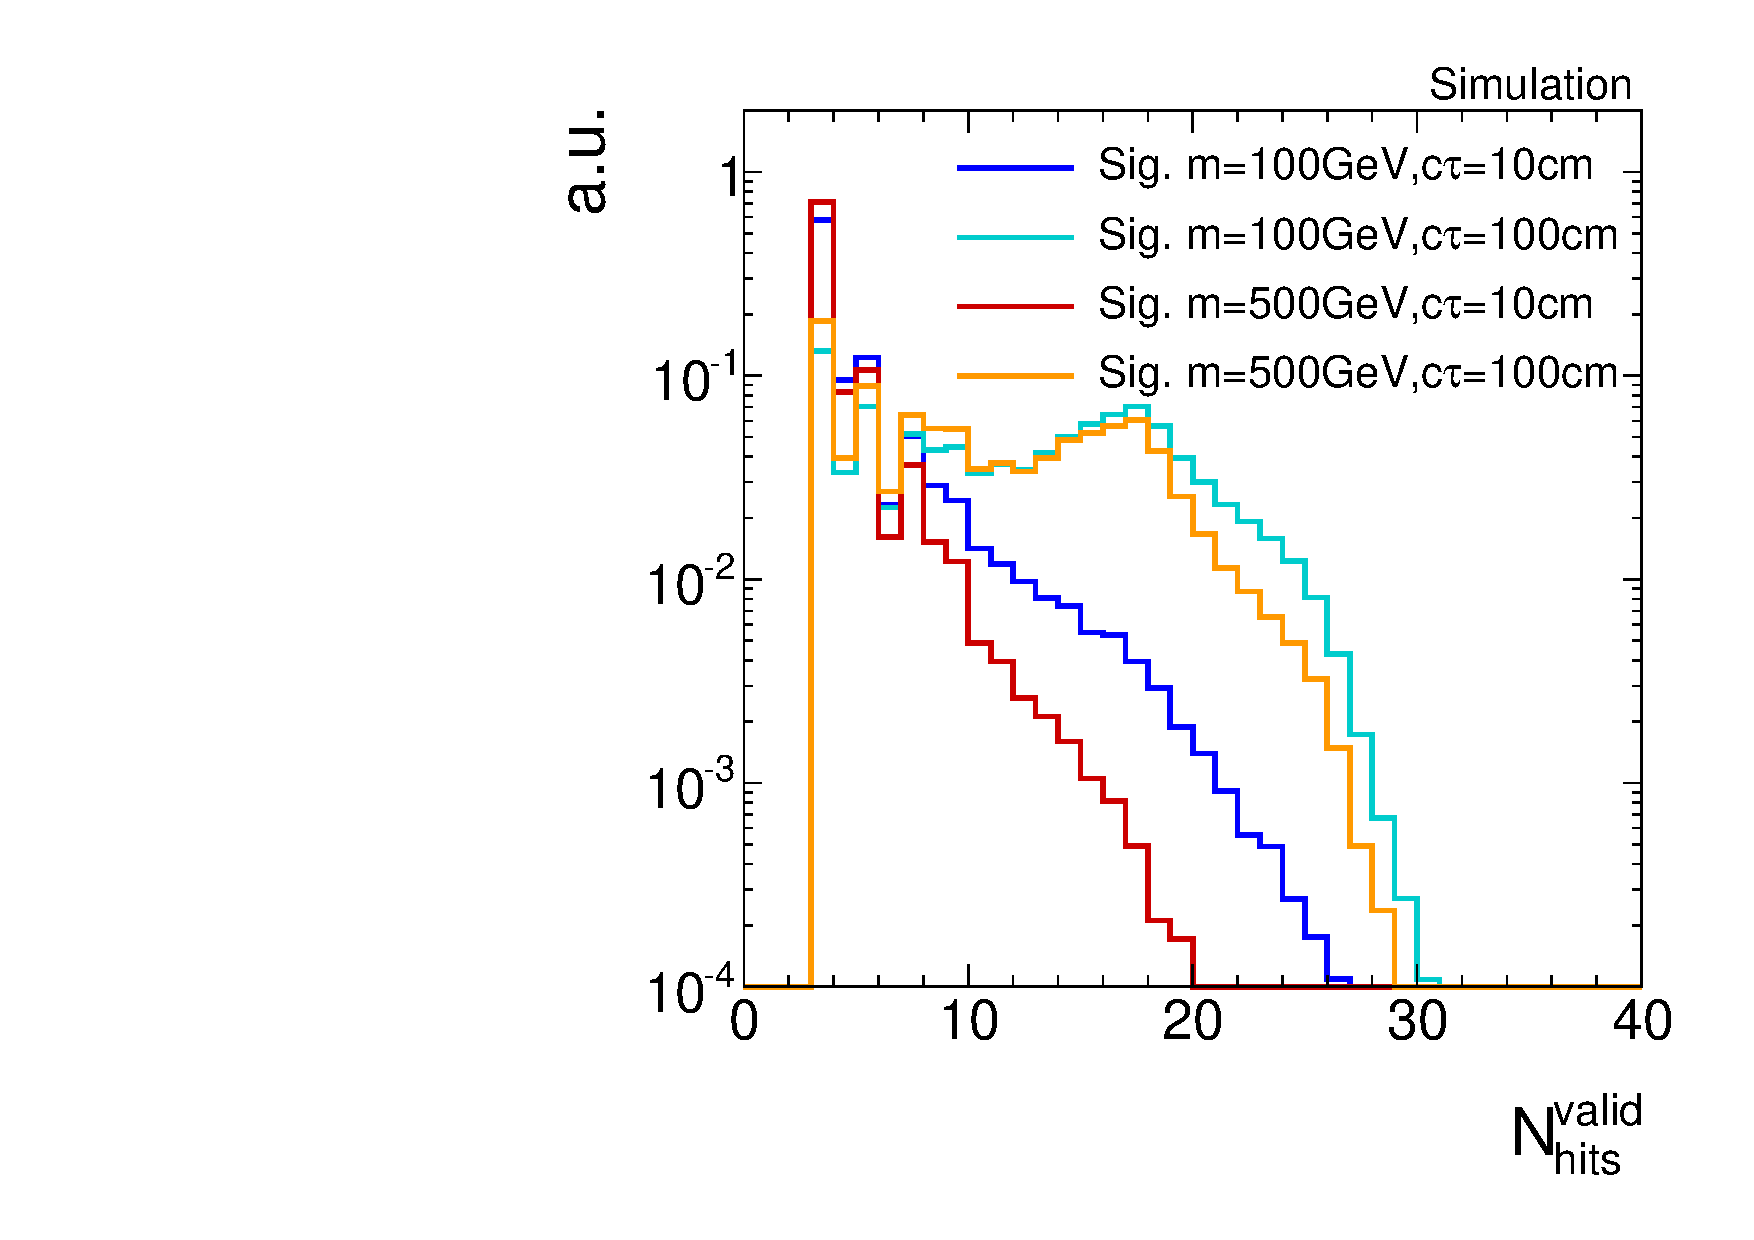
\includegraphics[width=0.49\textwidth]{figures/analysis_2/MotivationAndGeneralSearchStrategy/htrackNValid_log_chiTracksnoSelection.pdf}
  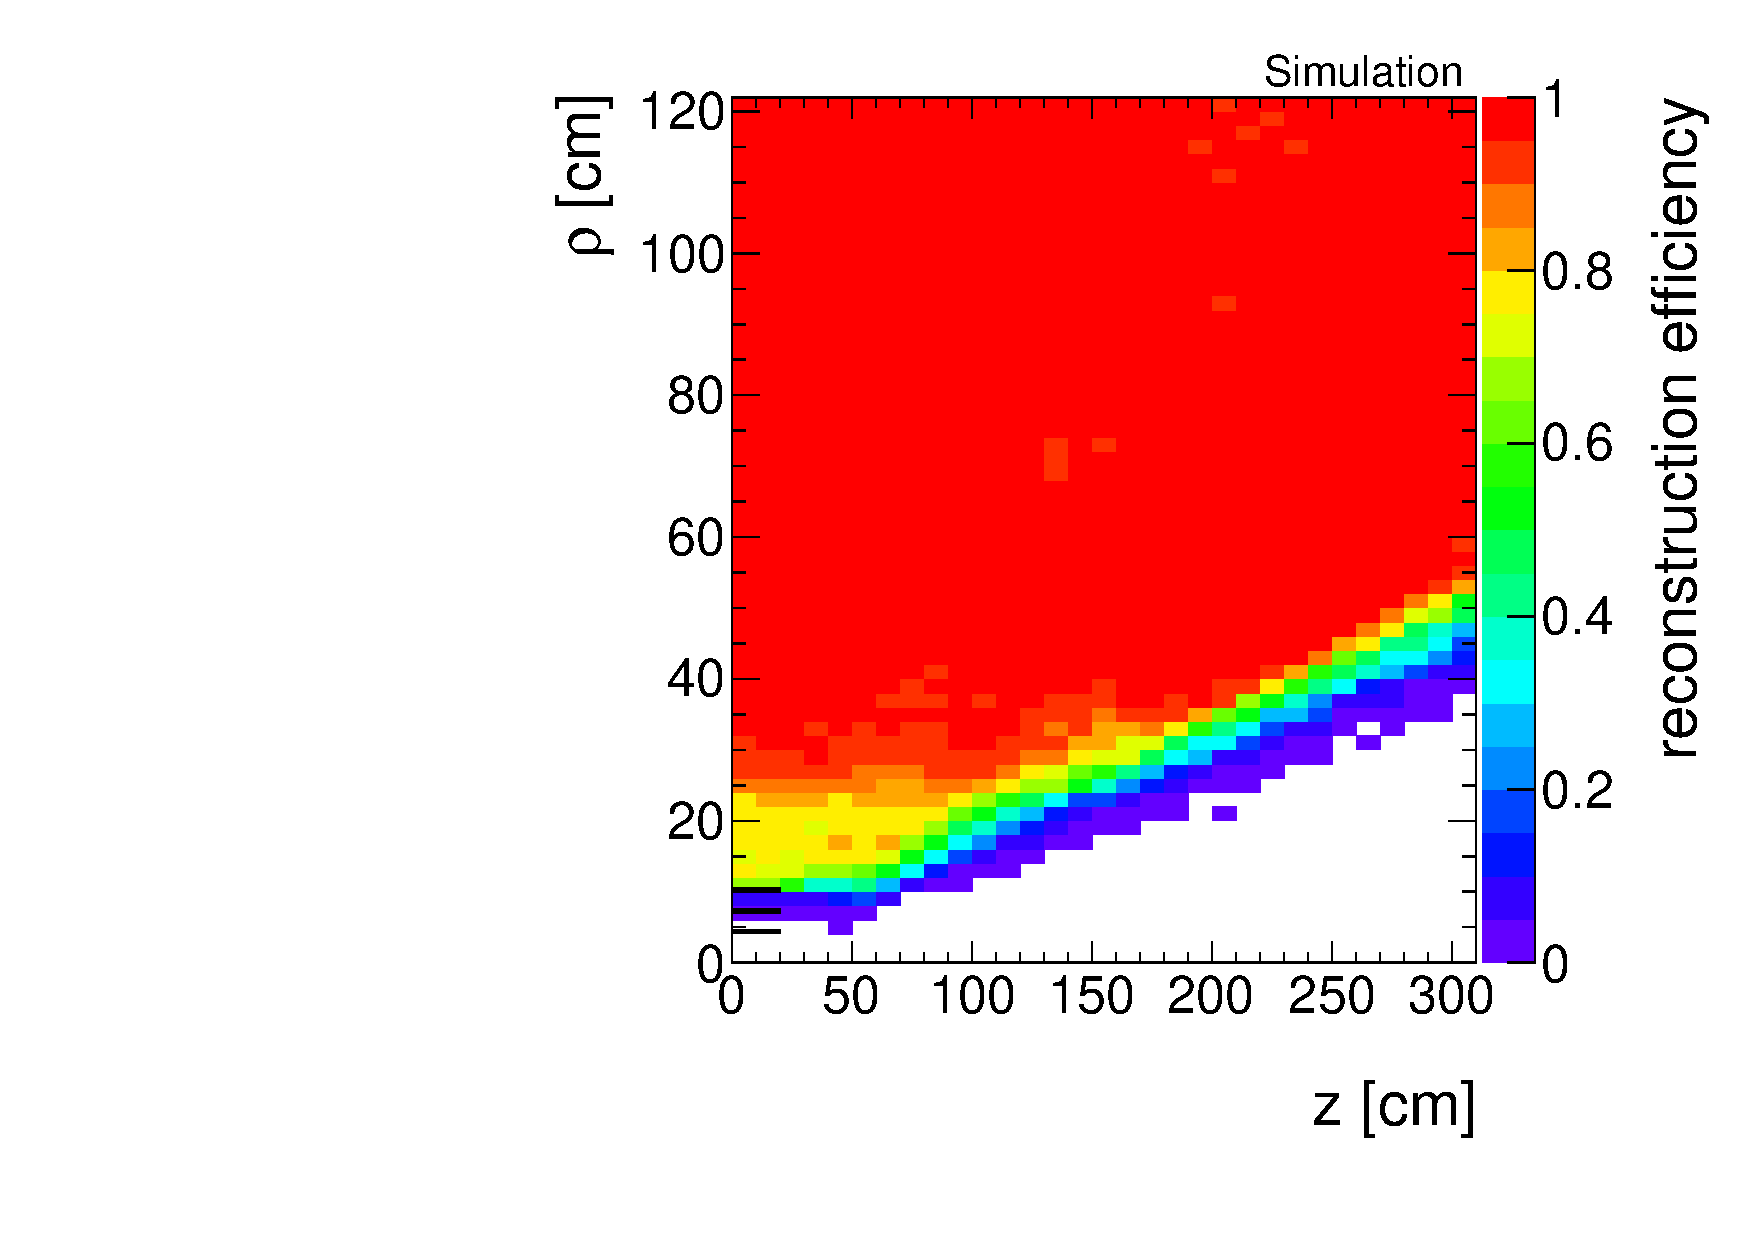
\includegraphics[width=0.49\textwidth]{figures/analysis_2/MotivationAndGeneralSearchStrategy/RecoEffTracksZoom.pdf}
  \end{tabular}
  \caption{FIXME: Left: Number of measurements in the tracker system \nhits for four different signal lifetimes.
           Right: Probability to reconstruct a track (z-axis) in dependency of the chargino's decay point in $z$-direction and radial direction $\rho = \sqrt{x^2 + y^2}$ (x- and y-axis).
           More information on the generation of the simulated signal samples can be found in Section~\ref{sec:SignalSamples}.} 
  \label{fig:NHits_2Signal_noSelection_normalized}
\end{figure}
FIXME: Since a minimum number of three hits are required to reconstruct a particle trajectory, there are no tracks with a lower number of measurements in the tracker system.
It can be seen, that \nhits peaks at the minimal possible value needed for track reconstruction of $\nhits=3$ for lower lifetimes.
%For higher lifetimes ($\ctau=50\cm$) the distribution shifts to higher values with a second peak at $\nhits\sim17$.
For a lifetime of $\ctau=100\cm$, a second peak at $\sim$17 hits appears corresponding to the number of measurements when crossing all pixel barrel (3) and strip inner and outer barrel (6 from stereo and 8 from normal) layers.
However, a notable fraction of $\sim$ 40\% of chargino tracks still has a number of measurements of $\nhits<8$. 

It should also be mentioned that the track reconstruction efficiency is sufficient for short chargino tracks so that loosening the \nhits requirement is expected to really improve the signal acceptance. 
The track reconstruction efficiency for different chargino decay points is depicted in Fig.~\ref{fig:NHits_2Signal_noSelection_normalized} (right).
For very short tracks ($\nhits=3$) the efficiency is still around 20\%.



Additionally, the search for disappearing tracks~\cite{bib:CMS:DT_8TeV} which targets models with charginos decaying inside the tracker did not make use of the high energy deposition of heavy particles. 
Although this variable was indeed used in the search for long-lived charged particles~\cite{bib:CMS:HSCP_8TeV}, this search was not optimised for intermediate lifetimes (\eg no explicit muon veto on the selected tracks was required). 
Thus, it shows less sensitivity compared to the disappearing track search in the lifetime region between $10\,\text{cm} \lesssim c\tau \lesssim 100\,\text{cm}$ (see Fig.~\ref{fig:pMSSMplot}).\\

To conclude, the general search strategy of the here presented analysis is to unite the strategies of~\cite{bib:CMS:HSCP_8TeV} and~\cite{bib:CMS:DT_8TeV} and to lower the strong selection on the number of hits in these analyses in order to get an optimised selection for lifetimes around $1\,\text{cm} \lesssim c\tau \lesssim  30\,\text{cm}$.

%%%%%%%%%%%%%%%%%%%%%%%%%%%%%%%%%%%%%%%%%%%%%%%%%%%%%%%%%%%%%%%%%%%%%%%%%%%%%%%%%%%%%%%%%%%%%%%%%%%%%%%%%%%%%%%%%%%%%%%%%%%%%%%%%%%%%%%%%%%%%%%%%%%%%%%%%%%%%%%%%%%%%%%%%%%%%%%%%%%%
%%%%%%%%%%%%%%%%%%%%%%%%%%%%%%%%%%%%%%%%%%%%%%%%%%%%%%%%%%%%%%%%%%%%%%%%%%%%%%%%%%%%%%%%%%%%%%%%%%%%%%%%%%%%%%%%%%%%%%%%%%%%%%%%%%%%%%%%%%%%%%%%%%%%%%%%%%%%%%%%%%%%%%%%%%%%%%%%%%%%
